\documentclass{article}

\title{ECE447 - Homework 4}
\author{Chase Lotito - SIUC Undergraduate}
\date{}

%% PACKAGES %%

\usepackage{amsmath, amsfonts, amssymb, amsthm}
\usepackage{braket}
\usepackage{listings}
\usepackage[margin=1.0in]{geometry}
\usepackage{xcolor}
\usepackage{textcomp}
\usepackage{graphicx}
\usepackage{fancyhdr}

%%%%%%%%%%%%%%

\graphicspath{{./images}}

%% LISTINGS CONFIG %%

\definecolor{purple2}{RGB}{153,0,153} % there's actually no standard purple
\definecolor{green2}{RGB}{0,153,0} % a darker green

\lstset{
  language=Python,                   % the language
  basicstyle=\normalsize\ttfamily,   % size of the fonts for the code
  frame = single,
  % Color settings to match IDLE style
  keywordstyle=\color{orange},       % core keywords
  keywordstyle={[2]\color{purple2}}, % built-ins
  stringstyle=\color{green2},%
  showstringspaces=false,
  commentstyle=\color{red},%
  upquote=true,                      % requires textcomp
}

\begin{document}

%%%%%%%%%%%%%%%%%%%%%
\pagestyle{fancy}

\maketitle

% attempt to make nice header
\fancyhead{}
\fancyhead[CH]{\normalsize{SOUTHERN ILLINOIS ECE / Chase Lotito / Spring 2024}}

\section{Problem 3.12}

I implemented the following plot for \(E_g(T)\) using python's library \textit{matplotlib.pyplot}.

\begin{lstlisting}{language = {Python}}
import matplotlib.pyplot as plt
import numpy as np
import math

# IMPORTANT CONSTANTS
Eg0 = 1.17          # Si bandgap at T=0K [eV]
alpha = 4.73e-4     # [eV/K]
beta = 636          # [K]

# define Eg(T) function
def bandgapTemp(T):
    """
    Calculate Si bandgap energy for a given temperature in K.
    Parameters:
    T = temp in K.
    """
    Eg = Eg0 - ( ( alpha * T**2 ) / (beta + T) )
    return Eg


##  Plotting ##

# Set up x-vals and input into Eg(T)
x = np.linspace(0, 600, 6000)
y = bandgapTemp(x)

markers_on = [3000]

# Create plot of Eg(T)
plt.plot(x, y, '-go', markevery=markers_on, label = "Eg(T)")

EgROOM = bandgapTemp(300)
plt.text((300 + 20), EgROOM, "(300, %.4f)" % EgROOM, fontsize = 12)

# Labels and Titles
plt.xlabel('Temperature (K)')
plt.ylabel('Bandgap Energy (eV)')
plt.title('Si Bandgap Energy v. Temperature')

# Axis Formatting
plt.xlim(0,600)

# Show plot
plt.legend()
plt.show()
\end{lstlisting}

\begin{figure}[!h] 
    \centering
    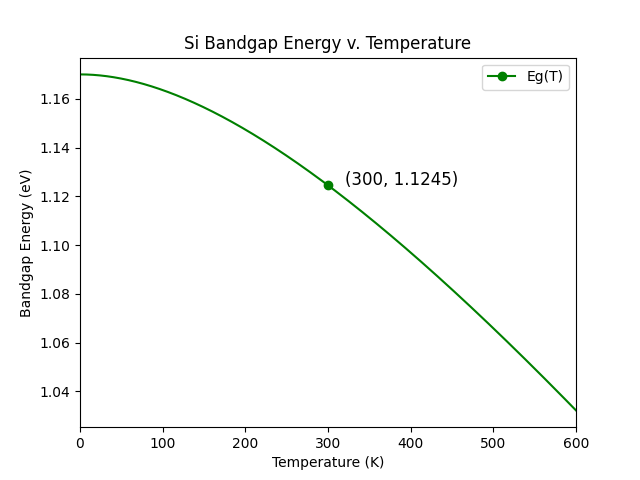
\includegraphics[width = 15cm]{bandgapTempPlot.png}
    \caption{\(E_G\) versus \(T\)}
    \label{fig:bandgapTemp}
\end{figure}

For \(T = 300K\), we see that the bangap energy of Silicon is 1.1245 eV, which is the textbook bandgap for Silicon at room temperature.

\end{document}
